\section*{Implementation}
	% IFØLGE JIM ER DET HER FISKEN HENTES TILBAKE PÅ LAND (BLANT ANDRE STEDER).
	% SE PÅ TØNNES SIN MASTEROPPGAVE FOR INSPIRASJON.
	
	DET SAMME SOM SEKSJONEN 'Benchmark'?
	\nl
	
	\tcol[blue]{WORKLOG-MATERIALE DANDERT I HENHOLD TIL GODE MASTER-THESES}
	\nl
	
	
	
	
	% PRØV Å HUSKE DET DU FORKLARTE TIL {SIGMUND}
	HUSK FINGRENE OG TIDSAKSEN PÅ BORDET (ISH DET SOM ER I FIGUREN UNDER FOR FASE, OG SÅ DET SAMME FOR FREKVENS-JUSTERING BARE MED F.EKS. HALVE—ELLER NOE ANNET— SOM START-FREKVENS; OG AT DE DA ENDER I "HARMONISK SYNKRONI").
	
	\begin{center}
	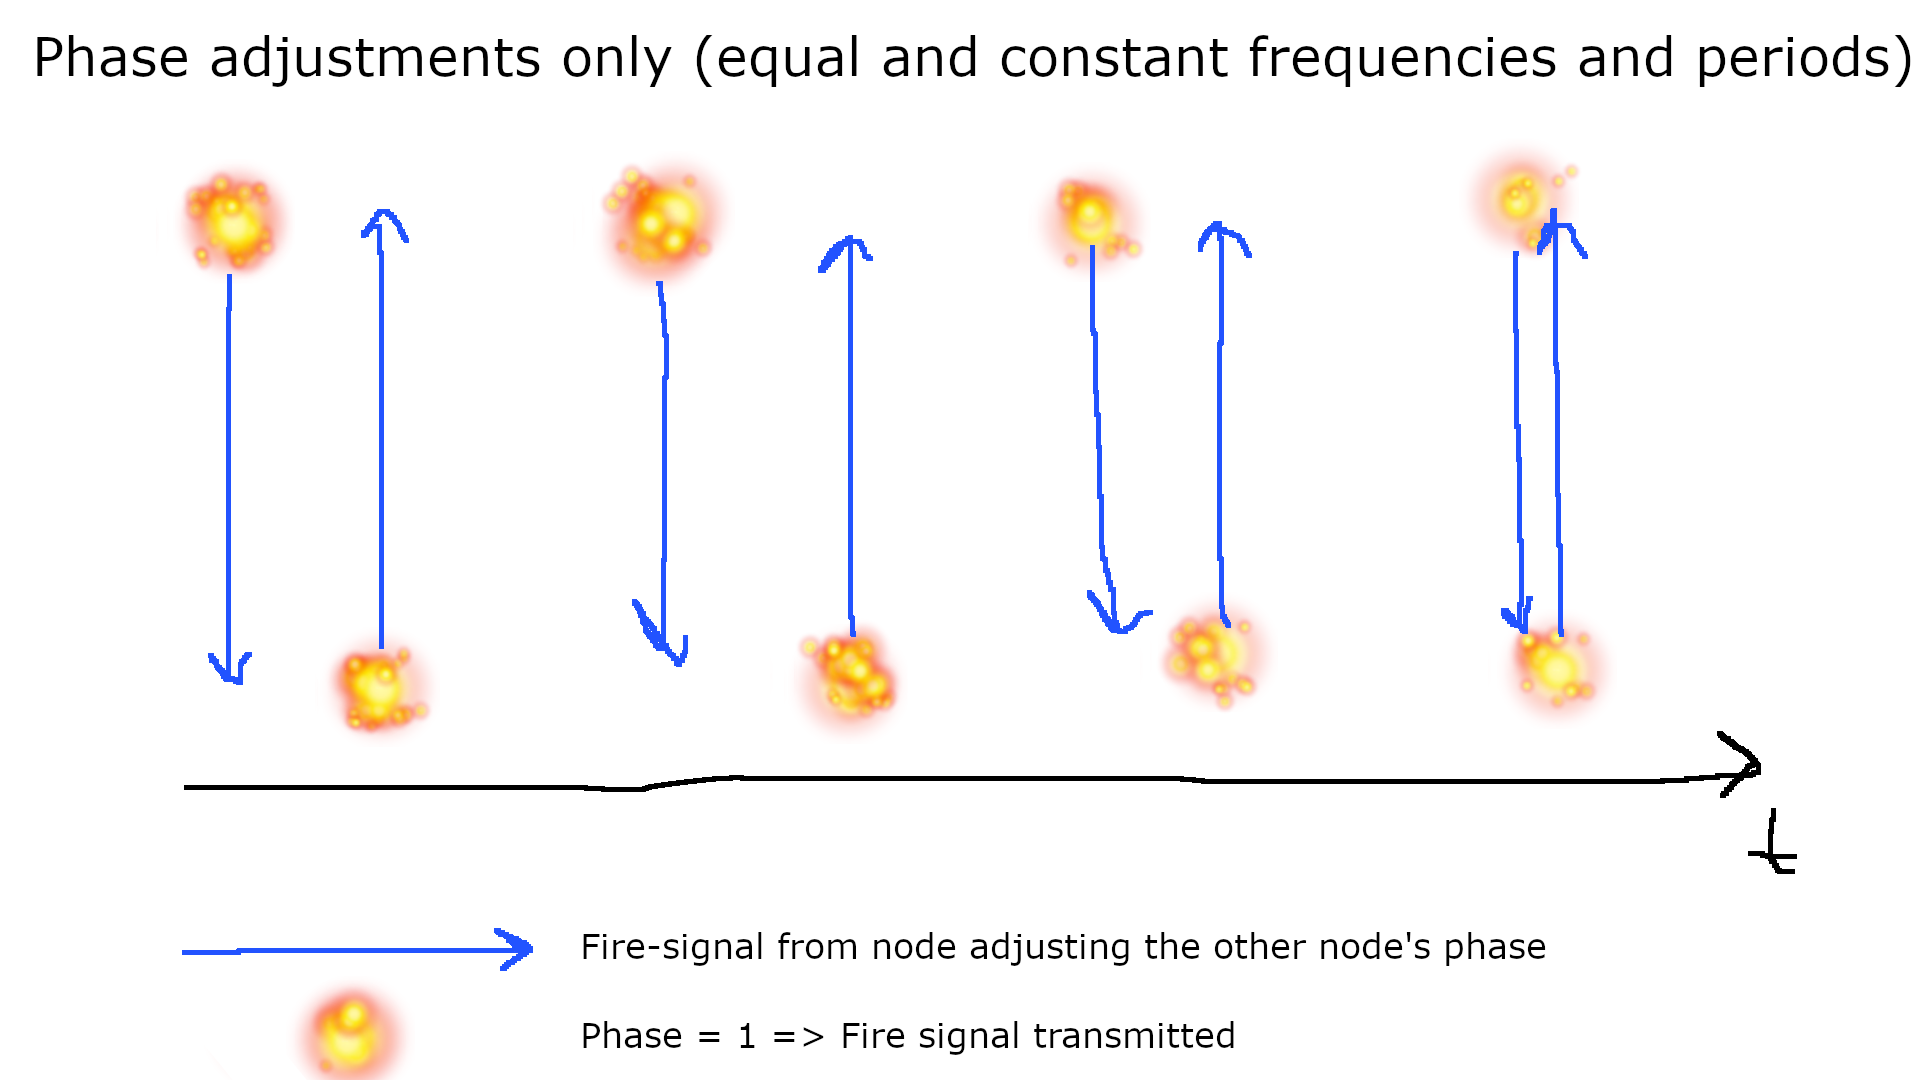
\includegraphics[width=0.90\textwidth]{Assets/Figures/phase_adjustments.png}
	\end{center}
	
	
	
	
	\tbf{FORKLARING TIL TANTE:}
	
	The diverse and complex phenomena of nature have for long served as exciting inspirations to human engineering and research (cite ant colonies, boids \& swarms, beeclust). One such phenomena studied and attempted modelled is the synchronous firing of fireflies in the rainforests.
	\nl
	
	* ILLUSTRATION OR PICTURE OF SYNCHRONIZING/SYNCHRONIZED FIREFLIES FIRING IN A DARK FOREST *
	\nl
	
	This has inspired scientists like Mirollo \& Strogatz (\tcol{citation}), and in later time Kristian Nymoen, Kyrre Glette et al. \cite{nymoen_synch}, to attempt to model and "etterlikne" this natural phenomenon in human-engineered systems. This work ties into the work on synchronizing oscillators (\tcol{citations?}) which has been subject to study for some time now. What separates Mirollo \& Strogatz and K. Nymoen's approach from these previous ones, is that here the oscillators are \tit{pulse-coupled}, as opposed to the more normal and constraining \tit{phase-coupled} (\tcol{explain?}).
	Each modelled "firefly", or firing node, is here implemented and considered as an oscillator, characterized by its phase and frequency. \tcol{Kinda, the job is to align sinusoidal waves, either by shifting an agent's phase "up", or "down".}
	\tcol{No training of any neural networks or any model-data was needed to achieve synchrony in this case — and so far no machine learning is used — but instead we see an emergent \tit{harmonic synchrony} in a collective, by endowing fairly simple agents with not too complicated update-functions. This is well known in the Multi-Agent Systems \& Swarm Robotics literature (citations?).}
	
	